% ATTENZIONE!!! 
% Per far funzionare i collegamenti ipertestuali si raccomanda di usare
%	\classname{nomedellaclasse}
% per le classi dello stesso package mentre invece 
%	\hyperref[nomedellaclasse]{\ttfamily{}nomequalificatodellaclasse}
% per le classi che non sono dello stesso package e che hanno il nome completo

% **************************************************
% Macro specifiche per il documento corrente
% **************************************************
% Nome
\newcommand{\docName}{Definizione di prodotto}
% Nome file
\newcommand{\docFileName}{definizione\_di\_prodotto.1.0.pdf}
% Versione
\newcommand{\docVers}{1.0}
% Data creazione
\newcommand{\creationDate}{2013-02-03}
% Data ultima modifica
\newcommand{\modificationDate}{2013-02-03}
% Stato in {Approvato, Non approvato}
\newcommand{\docState}{Non approvato}
% Uso in {Interno, Esterno}
\newcommand{\docUsage}{Esterno}
% Destinatari da specificare come nome1\\ &nome2\\ ecc.
\newcommand{\docDistributionList}{Prof. Tullio Vardanega\\&Prof. Riccardo Cardin\\&Dott. Gregorio Piccoli\\&Team SoftwareSynthesis}
% Redattori da specificare come nome1\\ &nome2\\ ecc.
\newcommand{\docAuthors}{Elena Zecchinato\\&Andrea Meneghinello\\&Riccardo Tresoldi}
% Approvato da
\newcommand{\approvedBy}{Andrea Rizzi}
% Verificatori
\newcommand{\verifiedBy}{Stefano Farronato\\&Marco Schivo}
% Perscorso (relativo o assoluto) che punta alla directory contenente shared/
% come sua sottodirectory (per comodità chiamiamola 'doc root').
\newcommand{\docRoot}{..}
% definire se si vuole l'indice delle tabelle
\def\INDICETABELLE{false}
% definire se si vuole l'indice delle figure
\def\INDICEFIGURE{false}

% importa il preambolo condiviso da tutti i documenti
% shared/preamble.tex
%
% Questo documento contiene la parte del preambolo condivisa e viene pertanto
% richiamato nel 'master' di tutti i documenti di progetto.  Al suo interno
% contiene le inclusioni (e le configurazioni) di tutti i package richiesti per
% la compilazione dei documenti, le macro di carattere generale e la definizione
% degli stili di pagina.

\documentclass[a4paper,10pt,openright]{article}

% **************************************************
% Macro generiche
% **************************************************
\newcommand{\team}{Software Synthesis}                    % chi siamo
\newcommand{\email}{software.synthesis@gmail.com}         % e-mail
\newcommand{\caName}{}                                    % titolo capitolato
\newcommand{\caDescr}{}                                   % descrizione
\newcommand{\inglese}[1]{\textit{#1}}

% **************************************************
% Codifica e lingua dei documenti
% **************************************************
\usepackage[utf8x]{inputenc}                              % codifica caratteri dei documenti sorgenti
\usepackage[english,italian]{babel}                       % localizzazione ai fini di sillabazione e cross-references
\usepackage[T1]{fontenc}                                  % codifica font di output

% **************************************************
% Definizione geometria della pagina
% **************************************************
\usepackage[a4paper,head=4cm,top=4.5cm,bottom=3cm,left=3cm,right=3cm,bindingoffset=5mm]{geometry}

% *************************************************
% Intestazioni e piè di pagina personalizzati
% *************************************************
\usepackage{fancyhdr}
% stile normale
\fancypagestyle{normal}{
\fancyhead{}                                              % intestazione
\fancyhead[RE,RO]{
\begin{picture}(0,0)
  \put(-410,0){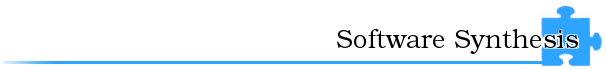
\includegraphics[width=1.02\textwidth]{header_logo}}
  \put(-410,10){\sffamily\large\leftmark}
\end{picture}
\vspace{-4pt}
}
\renewcommand{\headrulewidth}{.4pt}                       % riga sotto l'intestazione
\cfoot{}                                                  % piè di pagina
\fancyfoot[RO,LE]{\sffamily
  pag.~\thepage{} di \pageref{LastPage}}                  % a dx nelle pag. dispari e a sx in quelle pari
\fancyfoot[RE,LO]{\sffamily\docFileName{} -- v.\docVers}
\renewcommand{\footrulewidth}{.4pt}                       % riga sopra il piè di pagina
}
% stile per gli indici
\fancypagestyle{toc}{
\fancyhead{}                                              % intestazione
\fancyhead[RE,RO]{
\begin{picture}(0,0)
  \put(-410,0){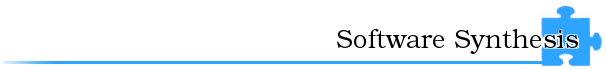
\includegraphics[width=1.02\textwidth]{header_logo}}
\end{picture}
}
\renewcommand{\headrule}{}                                % nessuna riga sotto l'intestazione
\cfoot{}                                                  % piè di pagina
\fancyfoot[RO,LE]{\sffamily\thepage{}}                    % a dx nelle pag. dispari e a sx in quelle pari
\fancyfoot[RE,LO]{\sffamily\docFileName{} -- v.\docVers}
\renewcommand{\footrulewidth}{.4pt}                       % riga sopra il piè di pagina
}

\pagestyle{fancy}                                         % premetto: non so usare bene le marche:
\renewcommand{\sectionmark}[1]{\markboth{#1}{#1}}         % se qualcuno ha idee migliori si faccia avanti!

% **************************************************
% Tabelle
% **************************************************
\usepackage{tabularx}                                     % tabelle di larghezza fissa con una o più colonne variabili
\usepackage{multirow}                                     % colonne con colonne che si estendono per più righe
\usepackage{booktabs}                                     % per inserire l'ambiente table e le righe orizz. nelle tabelle
\usepackage{longtable}			                          % tabelle oltre i limiti di pagina

% **************************************************
% Cross-references e collegamenti ipertestuali
% **************************************************
\usepackage[hidelinks]{hyperref}
\hypersetup{%
  colorlinks=false, linktocpage=false, pdfborder={0,0,0}, pdfstartpage=3, pdfstartview=FitV,%
  urlcolor=Cyan, linkcolor=Cyan, citecolor=Black, %pagecolor=Black,%
  pdftitle={\docName}, pdfauthor={\team}, pdfsubject={}, pdfkeywords={},%
  pdfcreator={pdflatex}, pdfproducer={pdflatex with hyperref package}%
}

% **************************************************
% Immagini e grafica
% **************************************************
\usepackage{graphicx}                                     % supporto ad aspetti avanzati delle immagini
\graphicspath{{\docRoot/pics/}}                           % percorso contenente tutti i file immagini
\usepackage{color}                                        % permette di colorare facilmente il testo

% **************************************************
% Altri pacchetti opzionali
% **************************************************     
\usepackage{lastpage}                                     % per sapere il numero totale di pagine
\usepackage{lipsum}                                       % genera "dummy text" per prove di impaginazione
\usepackage{eurosym}                                      % per il simbolo dell'euro usare \EUR{x} dove x è l'importo


% macro specifiche per il documento corrente
\newcommand{\classsection}[1]{\subsubsection{#1}\label{#1}}
\newcommand{\classname}[1]{\hyperref[#1]{\ttfamily#1}}

% Fine del preambolo e inizio del documento
\begin{document}

% Inclusione della prima pagina
% shared/firstpage.tex
%
% Questo documento definisce il contenuto della prima pagina, che si suppone
% essere uguale in tutti i documenti.  Oltre al logo e al titolo, la prima
% pagina contiene i metadati relativi al documento in cui viene inclusa.


% rimuove intestazioni e piè di pagina
\pagestyle{empty}

\begin{center}

% logo del gruppo

\includegraphics[width=1.5\textwidth]{logo}

\vspace{1in}

% titolo del documento
{\Huge\bfseries \docName}

\vspace{1in}

% tabella riepilogativa
\begin{tabularx}{.7\textwidth}{>{\bfseries\sffamily}l>{\sffamily}l}
\toprule
\multicolumn{2}{>{\sffamily}c}{Informazioni sul documento}\\
\midrule
Nome file:            & \docFileName\\
Versione:             & \docVers\\
Data creazione:       & \creationDate\\
Data ultima modifica: & \modificationDate\\
Stato:                & \docState\\
Uso:                  & \docUsage\\
Redattori:            & \docAuthors\\
Approvato da:         & \approvedBy\\
Verificatori:         & \verifiedBy\\
\bottomrule
\end{tabularx}

\end{center}

\newpage


%---------------------------RUOLI----------------------------
%FASE 1:
%Programmatori: DIEGO, STEFANO, SCHIVO
%FASE 2:
%Programmatori: MENE, TRES, ELENA

%Verificatore: SCHIVO, STEFANO, RIZZI, DIEGO (dobbiamo fare un sacco di test)
%Responsabile finale supremo: RIZZI
%------------------------------------------------------------

% Storico delle modifiche
\section*{Storia delle modifiche}
\begin{center}
\begin{longtable}{lp{.32\textwidth}lll}
\toprule
Versione & Descrizione intervento & Membro & Ruolo & Data\\
\midrule % inserire qui il contenuto della tabella
0.1 & Creazione del documento e stesura delle sezioni ``Introduzione'' e ``Riferimenti''. & &  & 2013-02-03\\
\bottomrule
\end{longtable}
\end{center}
\newpage

% inclusione dell'indice
% shared/toc.tex
%
% Questo file contiene le istruzioni che generano l'indice o gli indici del
% documento (utile nel caso in cui decidessimo di avere anche un indice delle
% tabelle e/o un indice delle figure).

\pagestyle{toc}
\pagenumbering{roman}

\tableofcontents

\newpage


% Alcuni aggiustamenti per le pagine
\pagenumbering{arabic}
\setcounter{page}{1}
\pagestyle{normal}

% Qui ha inizio il documento vero e proprio...
\newpage

\section{Introduzione}
\subsection{Scopo del prodotto}
\purpose

\subsection{Scopo del documento}
Il presente documento presenta una descrizione dettagliata dell'architettura del sistema software destinata a costituire il prodotto \caName{}, coerentemente con la progettazione ad alto livello contenuta nell'allegato \textit{specifica\_tecnica.2.0.pdf}.

A tal fine, si riporta per ognuno dei componenti definiti nel documento di specifica tecnica una descrizione delle classi in termini di operazioni disponibili, proprietà, responsabilità e collaborazioni. Il contenuto del presente documento ha inoltre valore vincolante per i programmatori, che avranno l'obbligo di attenersi alle disposizioni in esso contenute senza alcuna possibilità di deroga.

\subsection{Glossario}
\glossaryIntro

\subsection{Convenzioni di scrittura}
% vedere issue #56 al riguardo
Al fine di rendere quanto più agevole possibile la consultazione di questo documento da parte dei programmatori e del committente, è stata adottata una serie di accorgimenti sia a livello di riferimenti sulla nomenclatura delle classi sia a livello cromatico per campi dati e metodi. 
Tali norme possono essere consultate in dettaglio nel documento \textit{norme\_di\_progetto.3.0.pdf} allegato.
\clearpage

\section{Riferimenti}
\subsection{Normativi}
\begin{itemize}
\item[] \textit{piano\_di\_qualifica.3.0.pdf} allegato.
\item[] \textit{norme\_di\_progetto.3.0.pdf} allegato.
\item[] \textit{specifica\_tecnica.2.0.pdf} allegato
\end{itemize}

\subsection{Informativi}
\begin{itemize}
\item[] Capitolato d'appalto: \caName{}, v1.0, redatto e rilasciato dal proponente Zucchetti s.r.l. reperibile all'indirizzo \url{http://www.math.unipd.it/~tullio/IS-1/2012/Progetto/C1.pdf};
\item[] testo di consultazione: \textit{Software Engineering (8th edition) Ian Sommerville, Pearson Education | Addison Wesley};
\item[] manuale all'utilizzo dei design pattens: \textit{Design Patterns, Elementi per il riuso di software a oggetti -- (1/Ed. italiana) Eric Gamma, Richard Helm, Ralph Johnson, John Vlissides, Pearson Education};
\item[] \textit{glossario.3.0.pdf} allegato.
\end{itemize}
\clearpage

\section{Standard di progetto}

\subsection{Standard di progettazione architetturale}

\subsection{Standard di documentazione del codice}
% dobbiamo pensare se enumerarle qui oppure se rimandare a una sezione delle NdP
% vedere issue #54 al riguardo

\subsection{Standard di denominazione di entità e relazioni}

\subsection{Standard di programmazione}

\subsection{Strumenti di lavoro}

\clearpage

\section{Specifica sotto-architettura sever}\label{sec:serverarchitecture}

\subsection{Package org.softwaresynthesis.mytalk.server.dao}\label{sec:dao}

\classsection{IMessage}

\subsubsection*{Funzione}
L'interfaccia rappresenta un generico messaggio della segreteria.

\subsubsection*{Relazioni d'uso}

\subsubsection*{Metodi}
\begin{description}
	\item{\method{+ isNew(): boolean}}\\
Restituisce un valore booleano che fornisce le informazioni relative all'ascolto del messaggio: \texttt{true} se è stato ascoltato, \texttt{false} altrimenti.
	\item{\method{+ getSender(): IUserData}}\\
Restituisce il mittente del messaggio, sotto forma di un sottotipo (design pattern Proxy) di \classname{IUserData}.
	\item{\method{+ getDate(): Date}}\\
Restituisce la data di creazione del messaggio (appoggiandosi a \texttt{java.util.Date}).
	\item{\method{+ getLength(): int}}\\
Restituisce la lunghezza del messaggio espressa in secondi.
	\item{\method{+ getStream(): byte[]}}\\
Restituisce lo stream dati del messaggio.
	\item{\method{+ getSize(): int}}\\
Restituisce la dimensione del messaggio espressa in byte.
	\item{\method{+ setNew(value: boolean): void}}\\
Imposta il valore che determina se un messaggio è stato ascoltato o meno.

\end{description}

\classsection{AudioMessage}

\subsubsection*{Interfacce implementate}
\begin{itemize}[noitemsep,nolistsep]
  \item[-] \classname{IMessage}
\end{itemize}

\subsubsection*{Funzionalità}
La classe rappresenta il messaggio audio vero e proprio memorizzato nella segreteria dell'utente.

\subsubsection*{Relazioni d'uso}

\subsubsection*{Attributi}
\begin{description}
  \item{\memberdata{-- sender: IUserData}}\\
Riferimento all'utente che costituisce il mittente del messaggio audio.
  \item{\memberdata{-- date: Date}}\\
Data in cui è stato creato il messaggio audio.
  \item{\memberdata{-- path: String}}\\
Percorso che punta alla rappresentazione in forma persistente del messaggio audio.
  \item{\memberdata{-- new: boolean}}\\
Flag booleano che permette di discriminare i messaggi audio ascoltati da quelli non ascoltati.
  \item{\memberdata{-- content: byte[]}}\\
Rappresentazione del contenuto del messaggio audio.
\end{description}

\subsubsection*{Metodi}
Oltre alle implementazioni dell'interfaccia \classname{IAudioMessage}, la classe contiene i seguenti metodi:
\begin{description}
  \item{\method{AudioMessage(path: String)}}\\
Costruttore dell'oggetto \classname{AudioMessage}.
\end{description}

\classsection{AudioVideoMessage}

\subsubsection*{Interfacce implementate}
\begin{itemize}[noitemsep,nolistsep]
  \item[-] \classname{IMessage}
\end{itemize}

\subsubsection*{Funzionalità}
La classe rappresenta il messaggio audio/video vero e proprio memorizzato nella segreteria dell'utente.

\subsubsection*{Relazioni d'uso}

\subsubsection*{Attributi}
\begin{description}
  \item{\memberdata{-- sender: IUserData}}\\
Riferimento all'utente che costituisce il mittente del messaggio audio/video.
  \item{\memberdata{-- date: Date}}\\
Data in cui è stato creato il messaggio audio/video.
  \item{\memberdata{-- path: String}}\\
Percorso che punta alla rappresentazione in forma persistente del messaggio audio/video.
  \item{\memberdata{-- new: boolean}}\\
Flag booleano che permette di discriminare i messaggi audio/video ascoltati da quelli non ascoltati.
  \item{\memberdata{-- content: byte[]}}\\
Rappresentazione del contenuto del messaggio audio/video.
\end{description}

\subsubsection*{Metodi}
Oltre alle implementazioni dell'interfaccia \classname{IAudioVideoMessage}, la classe contiene i seguenti metodi:
\begin{description}
  \item{\method{AudioVideoMessage(path: String)}}\\
Costruttore dell'oggetto \classname{AudioVideoMessagio()}.
\end{description}

\classsection{IGroup}

\subsubsection*{Interfacce estese}
\begin{itemize}[noitemsep,nolistsep]
  \item[-] \hyperref[IContact]{\ttfamily{}org.softwaresynthesis.mytalk.abook.IContact}
\end{itemize}

\subsubsection*{Funzionalità}

\subsubsection*{Relazioni d'uso}

\subsubsection*{Metodi}
\begin{description}
	\item{\method{+ addContact(contact: IContact): void}}\\
Aggiunge al gruppo un nuovo oggetto IContact, può essere un sottogruppo oppure un singolo utente.
	\item{\method{+ getOwner(): IUserData}}\\
Restituisce l'utente proprietario del gruppo.
	\item{\method{+ getContact(): List<IContact>}}\\
Restituisce i contatti, sottogruppi oppure utenti, appartenenti al gruppo.
	\item{\method{+ setOwner(user: IUserData): void}}\\
Imposta l'utente proprietario del gruppo.
\end{description}

\classsection{StandardGroup}

\subsubsection*{Interfacce implementate}
\begin{itemize}[noitemsep,nolistsep]
  \item[-] \hyperref[IContact]{\ttfamily{}org.softwaresynthesis.mytalk.abook.IContact}
  \item[-] \classname{IGroup}
\end{itemize}

\subsubsection*{Funzionalità}

\subsubsection*{Relazioni d'uso}

\subsubsection*{Attributi}

\subsubsection*{Metodi}

\classsection{IUserData}
\subsubsection*{Interfacce estese}
\begin{itemize}[noitemsep,nolistsep]
  \item[-] \hyperref[IContact]{\ttfamily{}org.softwaresynthesis.mytalk.abook.IContact}
\end{itemize}

\subsubsection*{Funzionalità}

\subsubsection*{Relazioni d'uso}

\subsubsection*{Metodi}
\begin{description}
	\item{\method{+ getEMail(): string}}\\
Restituisce l'indirizzo e-mail con cui l'utente si è registrato.
	\item{\method{+ getPassword(): string}}\\
Restituisce la password, non criptata, dell'utente.
	\item{\method{+ getQuestion(): string}}\\
Restituisce la domanda, scelta dall'utente in fase di registrazione, per il recupero della password.
	\item{\method{+ getName(): string}}\\
Restituisce il nome dell'utente.
	\item{\method{+ getSurname(): string}}\\
Restituisce il cognome dell'utente.
	\item{\method{+ getPicture(): Image}}\\
Restituisce l'immagine che l'utente ha associato al proprio account.
	\item{\method{+ getAddressBook(): IAddressBook}}\\
Restituisce la rubrica dell'utente.
	\item{\method{+ getCallList(): List<ICall>}}\\
Restituisce la lista delle chiamate effettuate e ricevute dall'utente.
	\item{\method{+ getMessages(): List<IMessage>}}\\
Restituisce la lista di tutti i messaggi memorizzati nella segreteria dell'utente
	\item{\method{+ getMessages(news: Boolean): List<IMessage>}}\\
Restituisce la lista dei nuovi messaggi, in segreteria, se news è impostato a true altrimenti ritorna tutti quelli memorizzati.
	\item{\method{+ setEMail(mail: string): void}}\\
Imposta l'indirizzo e-mail di un utente.
	\item{\method{+ setPassword(password): void}}\\
Imposta la password che l'utente utilizza per accedere al sistema \caName.
	\item{\method{+ setQuestion(question: string): void}}\\
Imposta la domanda, scelta dall'utente utilizzata nella procedura di recupero della password.
	\item{\method{+ setAnswer(answer: string): void}}\\
Imposta la risposta alla domanda segreta utilizzata per la procedura di recupero della password.
	\item{\method{+ setName(name: string): void}}\\
Imposta il nome dell'utente.
	\item{\method{+ setSurname(surname: string): void}}\\
Imposta il cognome dell'utente.
	\item{\method{+ setPicture(image: Image): void}}\\
Imposta l'immagine relativa all'utente.
\end{description}

\classsection{StandardUserData}
\subsubsection*{Interfacce implementate}
\begin{itemize}[noitemsep,nolistsep]
  \item[-] \hyperref[IContact]{\ttfamily{}org.softwaresynthesis.mytalk.abook.IContact}
  \item[-] \classname{IUserData}
\end{itemize}

\subsection{Package org.softwaresynthesis.mytalk.server.connection}\label{sec:connection}

\classsection{ICommunicationHandler}

\subsubsection*{Funzionalità}

\subsubsection*{Relazioni d'uso}


\subsubsection*{Metodi}

\classsection{StandardCommunicationHandler}

\subsubsection*{Interfacce implementate}
\begin{itemize}[noitemsep,nolistsep]
  \item[-] \classname{ICommunicationHandler}
\end{itemize}

\subsubsection*{Funzionalità}

\subsubsection*{Relazioni d'uso}

\subsubsection*{Attributi}

\subsubsection*{Metodi}

\classsection{IConnection}

\subsubsection*{Funzionalità}

\subsubsection*{Relazioni d'uso}

\subsubsection*{Metodi}

\classsection{WebRTCInfo}

\subsubsection*{Interfacce implementate}
\begin{itemize}[noitemsep,nolistsep]
  \item[-] \classname{IConnection}
\end{itemize}

\subsubsection*{Funzionalità}

\subsubsection*{Relazioni d'uso}

\subsubsection*{Attributi}

\subsubsection*{Metodi}

\subsection{Package org.softwaresynthesis.mytalk.server.abook}\label{sec:abook}

\classsection{IContact}

\subsubsection*{Funzionalità}

\subsubsection*{Relazioni d'uso}

\subsubsection*{Metodi}
\begin{description}
  \item{\method{+ getName(): String}}\\
Restituisce il nome del contatto.
  \item{\method{+ setName(String name): void}}\\
Imposta il nome del contatto.
  \item{\method{+ getChildrenNumber(): int}}\\
Restituisce il numero di figli di un determinato nodo.
  \item{\method{+ addChild(contact: IContact): voi}}\\
Aggiunge un contatto (utente singolo o gruppo) come figlio del nodo selezionato.
  \item{\method{+ deleteChild(contact: IContact): void}}\\
Cancella dai figli del contatto di invocazione il contatto \texttt{contact}.
\end{description}

\classsection{IAddressBook}

\subsubsection*{Funzionalità}

\subsubsection*{Relazioni d'uso}

\subsubsection*{Metodi}

\classsection{AddressBook}

\subsubsection*{Interfacce implementate}
\begin{itemize}[noitemsep,nolistsep]
  \item[-] \classname{IAddressBook}
\end{itemize}

\subsubsection*{Funzionalità}

\subsubsection*{Relazioni d'uso}

\subsubsection*{Attributi}

\subsubsection*{Metodi}

\classsection{UserDataProxy}

\subsubsection*{Interfacce implementate}
\begin{itemize}[noitemsep,nolistsep]
  \item[-] \hyperref[IUserData]{\ttfamily{}org.softwaresynthesis.mytalk.server.dao.IUserData}
\end{itemize}

\subsubsection*{Funzionalità}

\subsubsection*{Relazioni d'uso}

\subsubsection*{Attributi}

\subsubsection*{Metodi}

\subsection{Package org.softwaresynthesis.mytalk.server.state}\label{sec:state}

\classsection{IState}

\subsubsection*{Funzionalità}

\subsubsection*{Relazioni d'uso}

\subsubsection*{Metodi}

\classsection{StateOnline}

\subsubsection*{Interfacce implementate}
\begin{itemize}[noitemsep,nolistsep]
  \item[-] \classname{IState}
\end{itemize}

\subsubsection*{Funzionalità}

\subsubsection*{Relazioni d'uso}

\subsubsection*{Attributi}

\subsubsection*{Metodi}

\classsection{StateOffline}

\subsubsection*{Interfacce implementate}
\begin{itemize}[noitemsep,nolistsep]
  \item[-] \classname{IState}
\end{itemize}

\subsubsection*{Funzionalità}

\subsubsection*{Relazioni d'uso}

\subsubsection*{Attributi}

\subsubsection*{Metodi}

\classsection{StateAvailable}

\subsubsection*{Interfacce implementate}
\begin{itemize}[noitemsep,nolistsep]
  \item[-] \classname{IState}
\end{itemize}

\subsubsection*{Funzionalità}

\subsubsection*{Relazioni d'uso}

\subsubsection*{Attributi}

\subsubsection*{Metodi}

\classsection{StateOccupied}

\subsubsection*{Interfacce implementate}
\begin{itemize}[noitemsep,nolistsep]
  \item[-] \classname{IState}
\end{itemize}

\subsubsection*{Funzionalità}

\subsubsection*{Relazioni d'uso}

\subsubsection*{Attributi}

\subsubsection*{Metodi}

\subsection{Package org.softwaresynthesis.mytalk.server.message}\label{sec:message}

\classsection{IMessageBox}

\subsubsection*{Funzionalità}

\subsubsection*{Relazioni d'uso}

\subsubsection*{Metodi}

\classsection{StandardMessageBox}

\subsubsection*{Interfacce implementate}
\begin{itemize}[noitemsep,nolistsep]
  \item[-] \classname{IMessageBox}
\end{itemize}

\subsubsection*{Funzionalità}

\subsubsection*{Relazioni d'uso}

\subsubsection*{Attributi}

\subsubsection*{Metodi}

\classsection{AudioMessageProxy}

\subsubsection*{Interfacce implementate}
\begin{itemize}[noitemsep,nolistsep]
  \item[-] \hyperref[IAudioMessage]{\ttfamily{}org.softwaresynthesis.mytalk.IAudioMessage}
\end{itemize}

\subsubsection*{Funzionalità}

\subsubsection*{Relazioni d'uso}

\subsubsection*{Attributi}
\begin{description}
  \item{\memberdata{-- sender: IUserData}}\\
Riferimento all'utente che costituisce il mittente del messaggio audio.
  \item{\memberdata{-- date: Date}}\\
Data in cui è stato creato il messaggio audio.
  \item{\memberdata{-- path: String}}\\
Percorso che punta alla rappresentazione in forma persistente del messaggio audio.
  \item{\memberdata{-- new: boolean}}\\
Flag booleano che permette di discriminare i messaggi audio ascoltati da quelli non ascoltati.
  \item{\memberdata{-- msg: AudioMessage}}\\
Riferimento di tipo \hyperref[AudioMessage]{\texttt{org.softwaresynthesis.mytalk.server.dao.AudioMessage}} al messaggio reale  costruito mediante la tecnica di lazy initialization.
\end{description}

\subsubsection*{Metodi}
Oltre alle implementazioni dell'interfaccia \texttt{org.mytalk.server.dao.IAudioMessage}, la classe prevede i seguenti metodi:
\begin{description}
\item{\method{+ AudioMessageProxy(path: String)}}\\
\end{description}

\classsection{AudioVideoMessageProxy}

\subsubsection*{Interfacce implementate}
\begin{itemize}[noitemsep,nolistsep]
  \item[-] \hyperref[IAudioVideoMessage]{\ttfamily{}org.softwaresynthesis.mytalk.IAudioVideoMessage}
\end{itemize}

\subsubsection*{Funzionalità}

\subsubsection*{Relazioni d'uso}

\subsubsection*{Attributi}
\begin{description}
  \item{\memberdata{-- sender: IUserData}}\\
Riferimento all'utente che costituisce il mittente del messaggio audio/video.
  \item{\memberdata{-- date: Date}}\\
Data in cui è stato creato il messaggio audio/video.
  \item{\memberdata{-- path: String}}\\
Percorso che punta alla rappresentazione in forma persistente del messaggio audio/video.
  \item{\memberdata{-- new: boolean}}\\
Flag booleano che permette di discriminare i messaggi audio/video ascoltati da quelli non ascoltati.
  \item{\memberdata{-- msg: AudioVideoMessage}}\\
Riferimento di tipo \hyperref[AudioVideoMessage]{\ttfamily{}org.softwaresynthesis.mytalk.server.dao.AudioVideoMessage} al messaggio reale costruito mediante la tecnica di lazy initialization.
\end{description}

\subsubsection*{Metodi}
Oltre alle implementazioni dell'interfaccia \hyperref[IAudioVideoMessage]{\ttfamily{}org.mytalk.server.dao.IAudioVideoMessage}, la classe prevede i seguenti metodi:
\begin{description}
\item{\method{+ AudioMessageProxy(path: String)}}\\
\end{description}

\subsection{Package org.softwaresynthesis.mytalk.server}\label{sec:server}

\classsection{IServerFacade}

\subsubsection*{Funzionalità}

\subsubsection*{Relazioni d'uso}

\subsubsection*{Metodi}

\classsection{StandardServerFacade}

\subsubsection*{Interfacce implementate}
\begin{itemize}[noitemsep,nolistsep]
  \item[-] \classname{IServerFacade}
\end{itemize}

\subsubsection*{Funzionalità}

\subsubsection*{Relazioni d'uso}

\subsubsection*{Attributi}

\subsubsection*{Metodi}

\clearpage

\section{Specifica sotto-archiettura clientpresenter}\label{clientpresenterarchitecture}

\subsection{Package org.softwaresynthesis.mytalk.clientpresenter}\label{sec:clientpresetner}

\classsection{IClient}

\subsubsection*{Funzionalità}

\subsubsection*{Relazioni d'uso}

\subsubsection*{Metodi}

\classsection{StandardClient}

\subsubsection*{Interfacce implementate}
\begin{itemize}[noitemsep,nolistsep]
  \item[-] \classname{IClient}
\end{itemize}

\subsubsection*{Funzionalità}

\subsubsection*{Relazioni d'uso}

\subsubsection*{Attributi}

\subsubsection*{Metodi}

\classsection{IPresenterFacade}

\subsubsection*{Funzionalità}

\subsubsection*{Relazioni d'uso}

\subsubsection*{Metodi}

\classsection{StandardPresenterFacade}

\subsubsection*{Interfacce implementate}
\begin{itemize}[noitemsep,nolistsep]
  \item[-] \classname{IPresenterFacade}
\end{itemize}

\subsubsection*{Funzionalità}

\subsubsection*{Relazioni d'uso}

\subsubsection*{Attributi}

\subsubsection*{Metodi}

\clearpage

\section{Specifica sotto-architettura clientview}\label{sec:clientviewarchitecture}

\subsection{Package org.softwaresynthesis.mytalk.clientview}\label{sec:clientview}

\classsection{IViewFacade}

\classsection{StandardViewFacade}

\subsection{Package org.softwaresynthesis.clientview.gui}\label{sec:gui}

\classsection{GUIHandler}

\classsection{AddressBookPanel}

\classsection{MainPanel}

\classsection{ToolsPanel}

\classsection{SearchResultPanel}

\classsection{ContactPanel}

\classsection{MessagePanel}

\classsection{LanguagePanel}

\classsection{AccountSettingsPanel}

\classsection{CallHistoryPanel}

\clearpage

\section{Tracciamento della relazione componenti-requisiti}

\end{document}
